\section{Methodology}
% \KZ{Here you can give a task description, which generalizes the BASIL dataset.
% You can say what is the input and output, that it being a binary classification
% problem etc. You can give one or two examples from Table 1 and leave the rest to
% experiment sec.}

Figure \ref{fig:model} illustrates our model MultiCTX (Multi-level ConTeXt). First, we carefully construct triplets from the original dataset and then apply supervised contrastive learning on them to obtain sentence embeddings. Second, we build relational sentence graphs by joining sentence nodes according to their discourse relationships and semantic similarity. Finally, we apply a Self-supervised Graph Attention Network \citep{kim2021how} to perform the bias detection as a node classification task. In essence, MultiCTX has two modules, Contrastive Learning Embedding (CSE) and Self-supervised Sentence Graph Attention Network (SSGAT). In order to investigate the role of the context and to imitate the way people learn from the news reports, we also apply a more reasonable and challenging cross-event data splitting. 

\subsection{Data splitting}

First of all, let's think about the nature of the news reports and the way people learn about the world in real life. News articles always emerge almost simultaneously in large numbers along with a particular event, over which people reason based on their experience learnt from previous events. Moreover, people usually read an article as a whole instead of randomly picking up several sentences and they are unlikely to encounter a sentence from news events happened before. Additionally, people tend to collect information from more than one article to get a bigger picture of the new event. Therefore, in order to simulate the real human's learning process, different from the commonly-used data splitting which randomly distributes sentences to one of the three subsets (train/val/test), we use event-wise data splitting mentioned in \citet{van-den-berg-markert-2020-context}, \citet{chen-etal-2020-detecting}. We treat the articles reporting the same event as a unit and keeping sentences from the same event in the same subset. Part of the data is shown in Table \ref{tab:basil} with clear `adjacent sentences', `article' and `event' structure.

Furthermore, splitting by events is more reasonable and more demanding, in terms of model generalizability for identifying informational bias from unseen events. Experiments in \citet{van-den-berg-markert-2020-context} and \citet{chen-etal-2020-detecting} also show that common models including BERT-based models all experienced a considerable performance drop when switching from random splitting to event-based splitting.

\begin{table*}[th]
    \centering
    \begin{tabular}{cccp{12cm}c}
        \toprule
        \textbf{Event} & \textbf{Source} & \textbf{Index} & \textbf{Sentence} & \textbf{Label} \\
        \midrule
        86 & nyt & 3 &  Officials said Mr. Mattis went to the White House with his resignation letter already written, but nonetheless made a last attempt at persuading the president to reverse his decision about Syria, which Mr. Trump announced on Wednesday over the objections of his senior advisers. & 0\\
        \hline
        86 & nyt & 4 &  Mr. Mattis, a retired four-star Marine general, was rebuffed. & 1\\
        \hline
        86 & nyt & 5 &  Returning to the Pentagon, he asked aides to print out 50 copies of his resignation letter and distribute them around the building. & 0 \\
        \midrule
        11 & fox & 20 & However, Democrats rejected the plan even before Trump announced it, and a Senate version of the plan failed to get the 60 votes needed on Thursday.  & 1\\
\hline
        11 & fox & 21 & A second bill, already passed by the Democrat-controlled House to re-open the government, also fell short. & 0\\
        \midrule
        2 & hpo & 10 & There were roughly 520,000 arrests for unauthorized border crossings last year, which is about one-third of the 1.6 million arrests that happened in 2000. & 0\\
        \hline
        2 & hpo & 11 &Since 2014, a high proportion of those crossing have been Central American children and families seeking to make humanitarian claims such as asylum. & 1\\
        \bottomrule
    \end{tabular}
    \caption{BASIL dataset}
    \label{tab:basil}
\end{table*}


\subsection{Sentence Embedding using Contrastive Learning}

The idea of contrastive learning is that humans discriminate objects by ``comparison'', thus similar objects should be close to each other in the representation space, and different objects should be as far apart as possible. However, news sentences inherently have small differences in terms of pure text. Two sentences with opposite stances might be different in a few words, while two sentences expressing the
same idea are likely to be formulated completely differently. To address the problem, we apply supervised contrastive learning with hard negatives described in \citet{gao2021simcse}. The idea is to develop, from the original dataset, the triplets $(x_i,x^+_i,x^-_i)$  each denotes target sentence, positive sample and negative sample respectively. Using the $\mathbf{h}_{i},\mathbf{h}_{i^+},\mathbf{h}_{i}^-$ representations of $x_i,x^+_i,x^-_i$, 
the objective function to minimize is InfoNCE Loss. 

% \begin{align}
% l_i = -\log \frac{e^{\operatorname{sim}\left(\mathbf{h}_{i}, \mathbf{h}_{i}^{+}\right) / \tau}}{\sum\limits_{j=1}^{\text{batch size}}\left(e^{\operatorname{sim}\left(\mathbf{h}_{i}, \mathbf{h}_{j}^{+}\right) / \tau}+e^{\operatorname{sim}\left(\mathbf{h}_{i}, \mathbf{h}_{j}^{-}\right) / \tau}\right)}
% \end{align}

The difficulty is to mine the positive and negative samples for each target sentence from the original dataset. A good positive sample is supposed to capture the most essential features of the sentence, rather than being influenced by other factors, such as the writing styles of different news media. Therefore, the best positive sample is expected to be significantly different from the target sample in terms of sentence formation, while the best negative sample should be similar to the target sentence in terms of syntactic structure. In short, samples with different labels from the target sentence but with initial embedding in its vicinity are likely to be the most useful, providing significant gradient information during the training process.

Inspired by \citet{baly-etal-2020-detect} which applies a triplet loss in training using news media in triplet selection, our final triplet follows article-based criteria and is composed of: $x_i$: target sentence; $x_i^+$: same label and event with $x_i$, but from a different article; $x_i^-$: from the same article with $x_i$ but with a different label. Figure \ref{fig:triplet} illustrates our triplet construction.

Thereby we essentially augment the original 7977-sentence corpus to a much larger dataset of around 300k triplets where sentences are no longer isolated but linked to two others. More importantly, triplets with the same target sentence provide altogether a `context' to help its representational learning. This context integrates two advantages: 1) it provides article-level contextual information from the same article by the negative sample, and also event-level context from other articles of the same event; 2) it discourages the model to learn from superficial writing styles of the article or the news publisher. Our experiments also confirmed that this article-based triplet construction is better than either the news outlet-based triplet or the event-based one.

%  which achieves data enhancement in a certain sense. Moreover, since the ternary set is constructed using news articles under the same event (negative samples from the same article, and positive samples from different news sources but the same event), the model can not only exclude the influence of different news media writing styles in the process of comparative learning, and learn more essential content beyond rhetorical sentence construction, but also learn the contextual knowledge of the event described by the target text. This process simulates the process of receiving news and making judgments in the real world.




% 说一下按比例分布?有多少数据点?
% 画个图(降维之后)?
% In addition, in order to make the training samples cover the whole training set, this study constructs a sampling distribution that proportionalizes the sampling frequency to the number of available positive and negative samples to ensure that the final triad distribution is similar to the distribution of the original dataset.

\begin{figure}[!htbp]\centering
    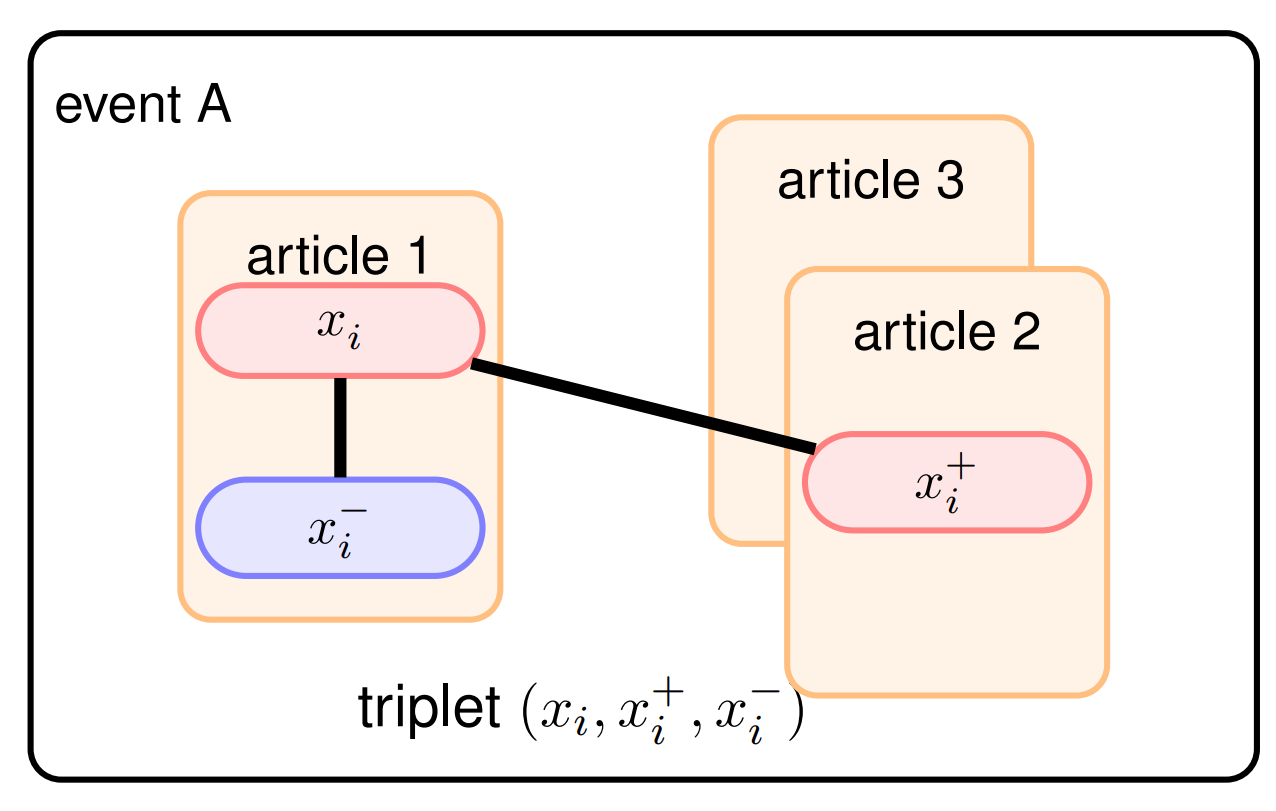
\includegraphics[width=.7\linewidth]{img/triplet.PNG}
      \caption{Triplet construction. Positive sample $x_i^+$ has same label (red) and event with target sentence $x_i$; negative sample $x_i^-$ has different label (blue) but from the same article with $x_i$; note that three sentences must from same event.}
  \label{fig:triplet}
\end{figure}

% \begin{figure}[!htbp]\centering
%     \begin{tikzpicture}
%       [scale=.5, transform shape, 
%       event/.style = {rectangle,rounded corners, minimum width=230pt, minimum height = 140pt, draw = black, fill = white, thick},
%       vertex/.style = {rounded rectangle, minimum width=60pt, minimum height = 17pt, draw=red!50, fill = red!10, thick},
%       article/.style = {rectangle,rounded corners,minimum width=60pt, minimum height = 80pt, draw = orange!50, fill = orange!10, thick}, 
%       neg/.style = {rounded rectangle, minimum width=60pt, minimum height = 10pt, draw=blue!50, fill = blue!10, thick},
%       textbox/.style = {rectangle, minimum width=60pt, minimum height = 20pt},
%       edge_style/.style={draw=black, ultra thick}]
%       \node[event][fill=white] (n0) at (3,4)  {};
%       \node[textbox] at (2.6,2) {\large triplet $(x_i,x^+_i,x^-_i)$};
      
%       \node[article] (n1) at (1,4)  {};
%       \node[textbox] at (1,5) {article 1};
      
%       \node[article] (n2) at (4.5,4.5)  {};
%       \node[textbox] at (4.5,5.5) {article 3};

%       \node[article] (n3) at (5,3.5)  {};
%       \node[textbox] at (5,4.5) {article 2};
%       \node[vertex] (n4) at (1,4.5)  { $x_i^{ }$ };
%       \node[neg] (n5) at (1,3.2)  { $x_i^-$ };
%       \node[vertex] (n6) at (5,3.5)  { $x_i^+$ };
%       \node[textbox] at (-0.3,6) {event A};
%       \foreach \from \to /\weight in {n4/n5/,n4/n6/}
%         \draw[edge_style] (\from) -- node {\weight}(\to);
   
%     \end{tikzpicture}
%   \caption{Triplet construction. Positive sample $x_i^+$ has same label (red) and event with target sentence $x_i$; negative sample $x_i^-$ has different label (blue) but from the same article with $x_i$; note that three sentences must from same event.}
%   \label{fig:triplet}
% \end{figure}

% The difficulty of triplet loss is to mine the hard sampling. Take character recognition as an example: the same person, with different posture, or dress change, this is the hard positive sample. Two different people, wearing the same clothes and shooting from the same angle, is a hard negative sample.

% The purpose is to reduce the distance between similar things and increase the distance between different classes, so as to obtain a better representation vector for the text.

% by minimizing $\max (D(h,h^+)-D(h,h^-)+\alpha,0)$
% The performance of the sentence embedding obtained through contrastive learning is better already than that of BERT and LSTM by directly bifurcating it with the most basic logistic regression.

\subsection{Relational Sentence Graph}

Sentences are naturally suitable as nodes when encoding long documents, so we borrowed the idea from extractive text summarization from \citet{christensen-etal-2013-towards} and \citet{summpip} to construct graphs. The graphs are formed by connecting the sentences in four different ways illustrated in \ref{subfig:edgetype}:

\begin{enumerate} \label{para:edge}
    \item Deverbal noun reference: when an action in verb form occurs in the current sentence, it is likely to be mentioned in the noun form in the following sentences. So we attach the current sentence with its downstream sentence when at least one semantically similar deverbal noun is found in the latter.
    
    \item Discourse marker: If the immediately subsequent sentence begins with a discourse marker (e.g., however, meanwhile, furthermore), the two sentences are linked.
    
    \item Entity continuation: we connect two sentences in the same event if they contain the same entity.
    
    \item Sentence similarity: sentence pairs in the same event with high cosine similarity are joined.
    
\end{enumerate}

% 画个图,从真实数据里找句子, 找个event画一下 yes
% edge typeeeeeeeeeeeeeeeeeeeeeeee

\begin{figure}[!htbp]\centering

    \subfigure[Four types of edges in relational sentence graph. \underline{Underline}: deverbal noun reference; \textit{italic}: discourse maker; \textbf{bold}: entity continuation; \textcolor{blue!60}{colored}: sentence similarity]{
    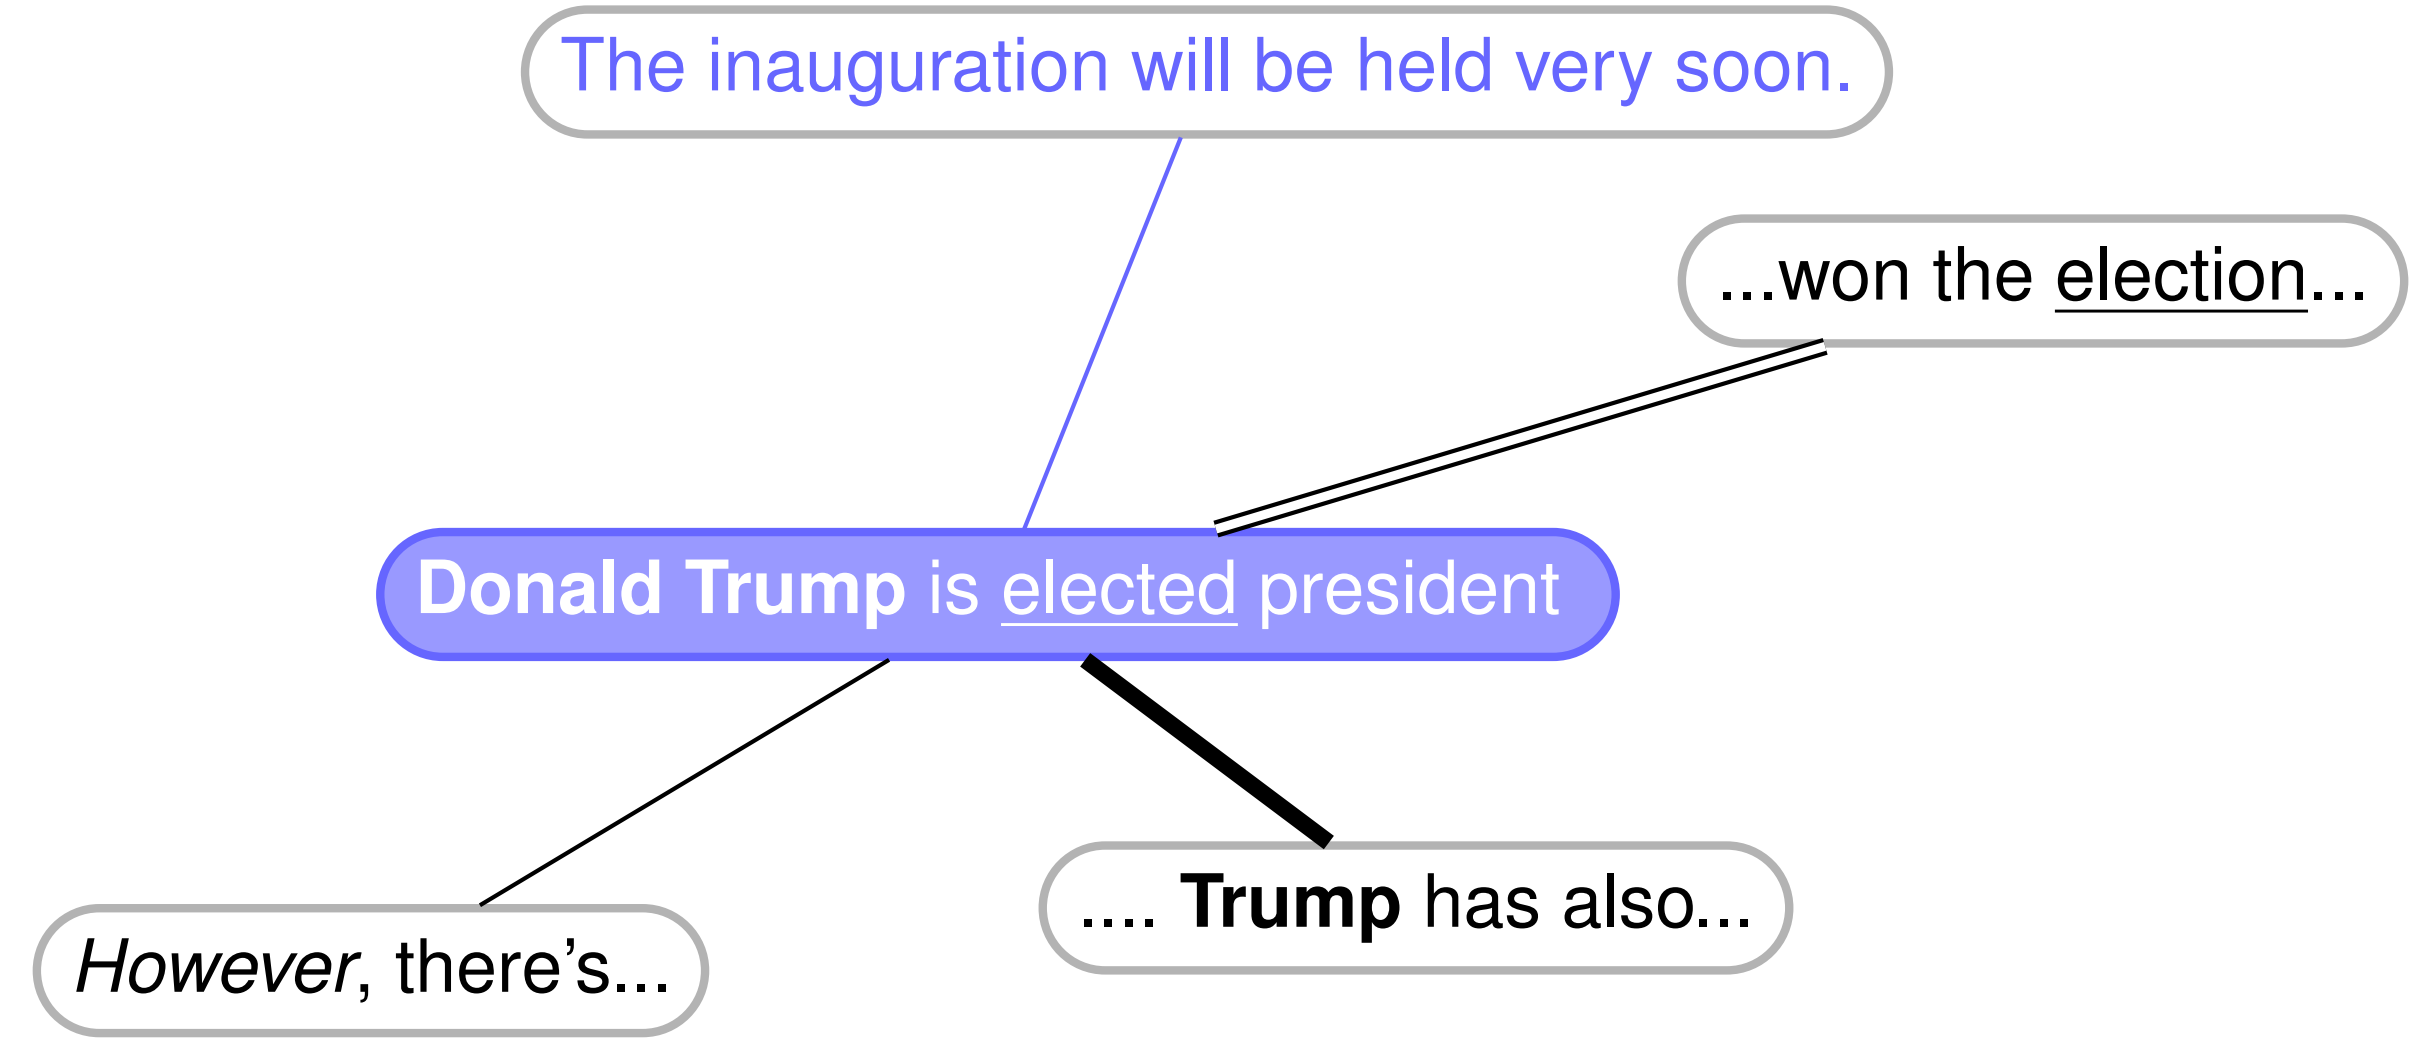
\includegraphics[width=.8\linewidth]{img/edgetype.PNG}
%     \begin{tikzpicture}
%       [scale=.6, transform shape,
%       vertex/.style = {rounded rectangle, minimum width=60pt, minimum height = 17pt, draw = black!30, thick},
%       textbox/.style = {rectangle, minimum width=60pt, minimum height = 20pt},
%       edge_style/.style={draw=black, ultra thick}]
%         \node[vertex] (n2) at (2,6)  {\textcolor{blue!60}{The inauguration will be held very soon.} };
%     \node[vertex] (n3) at (3,2)  { .... \textbf{Trump} has also...};
%       \node[vertex][draw=blue!60, fill = blue!40] (n4) at (1,3.5)  { \textcolor{white}{\textbf{Donald Trump} is \underline{elected} president }};
%       \node[vertex] (n5) at (-2,1.7)  { \textit{However}, there's... };
%       \node[vertex] (n6) at (6,5)  {...won the \underline{election}... };
%     %   \node[textbox] at (4.5,1.3) {event A};
%       \foreach \from \to /\weight in {n4/n5/}
%         \draw[draw=black] (\from) -- node {\weight}(\to);
%     \foreach \from \to /\weight in {n4/n6/}
%         \draw[draw=black, double distance=.03cm] (\from) -- node {\weight}(\to);
%   \foreach \from \to /\weight in {n4/n2/}
%         \draw[draw=blue!60] (\from) -- node {\weight}(\to);
%   \foreach \from \to /\weight in {n4/n3/}
%         \draw[edge_style] (\from) -- node {\weight}(\to);
%     \end{tikzpicture}
      \label{subfig:edgetype}
    }
  \subfigure[nodes are colored by news source]{
    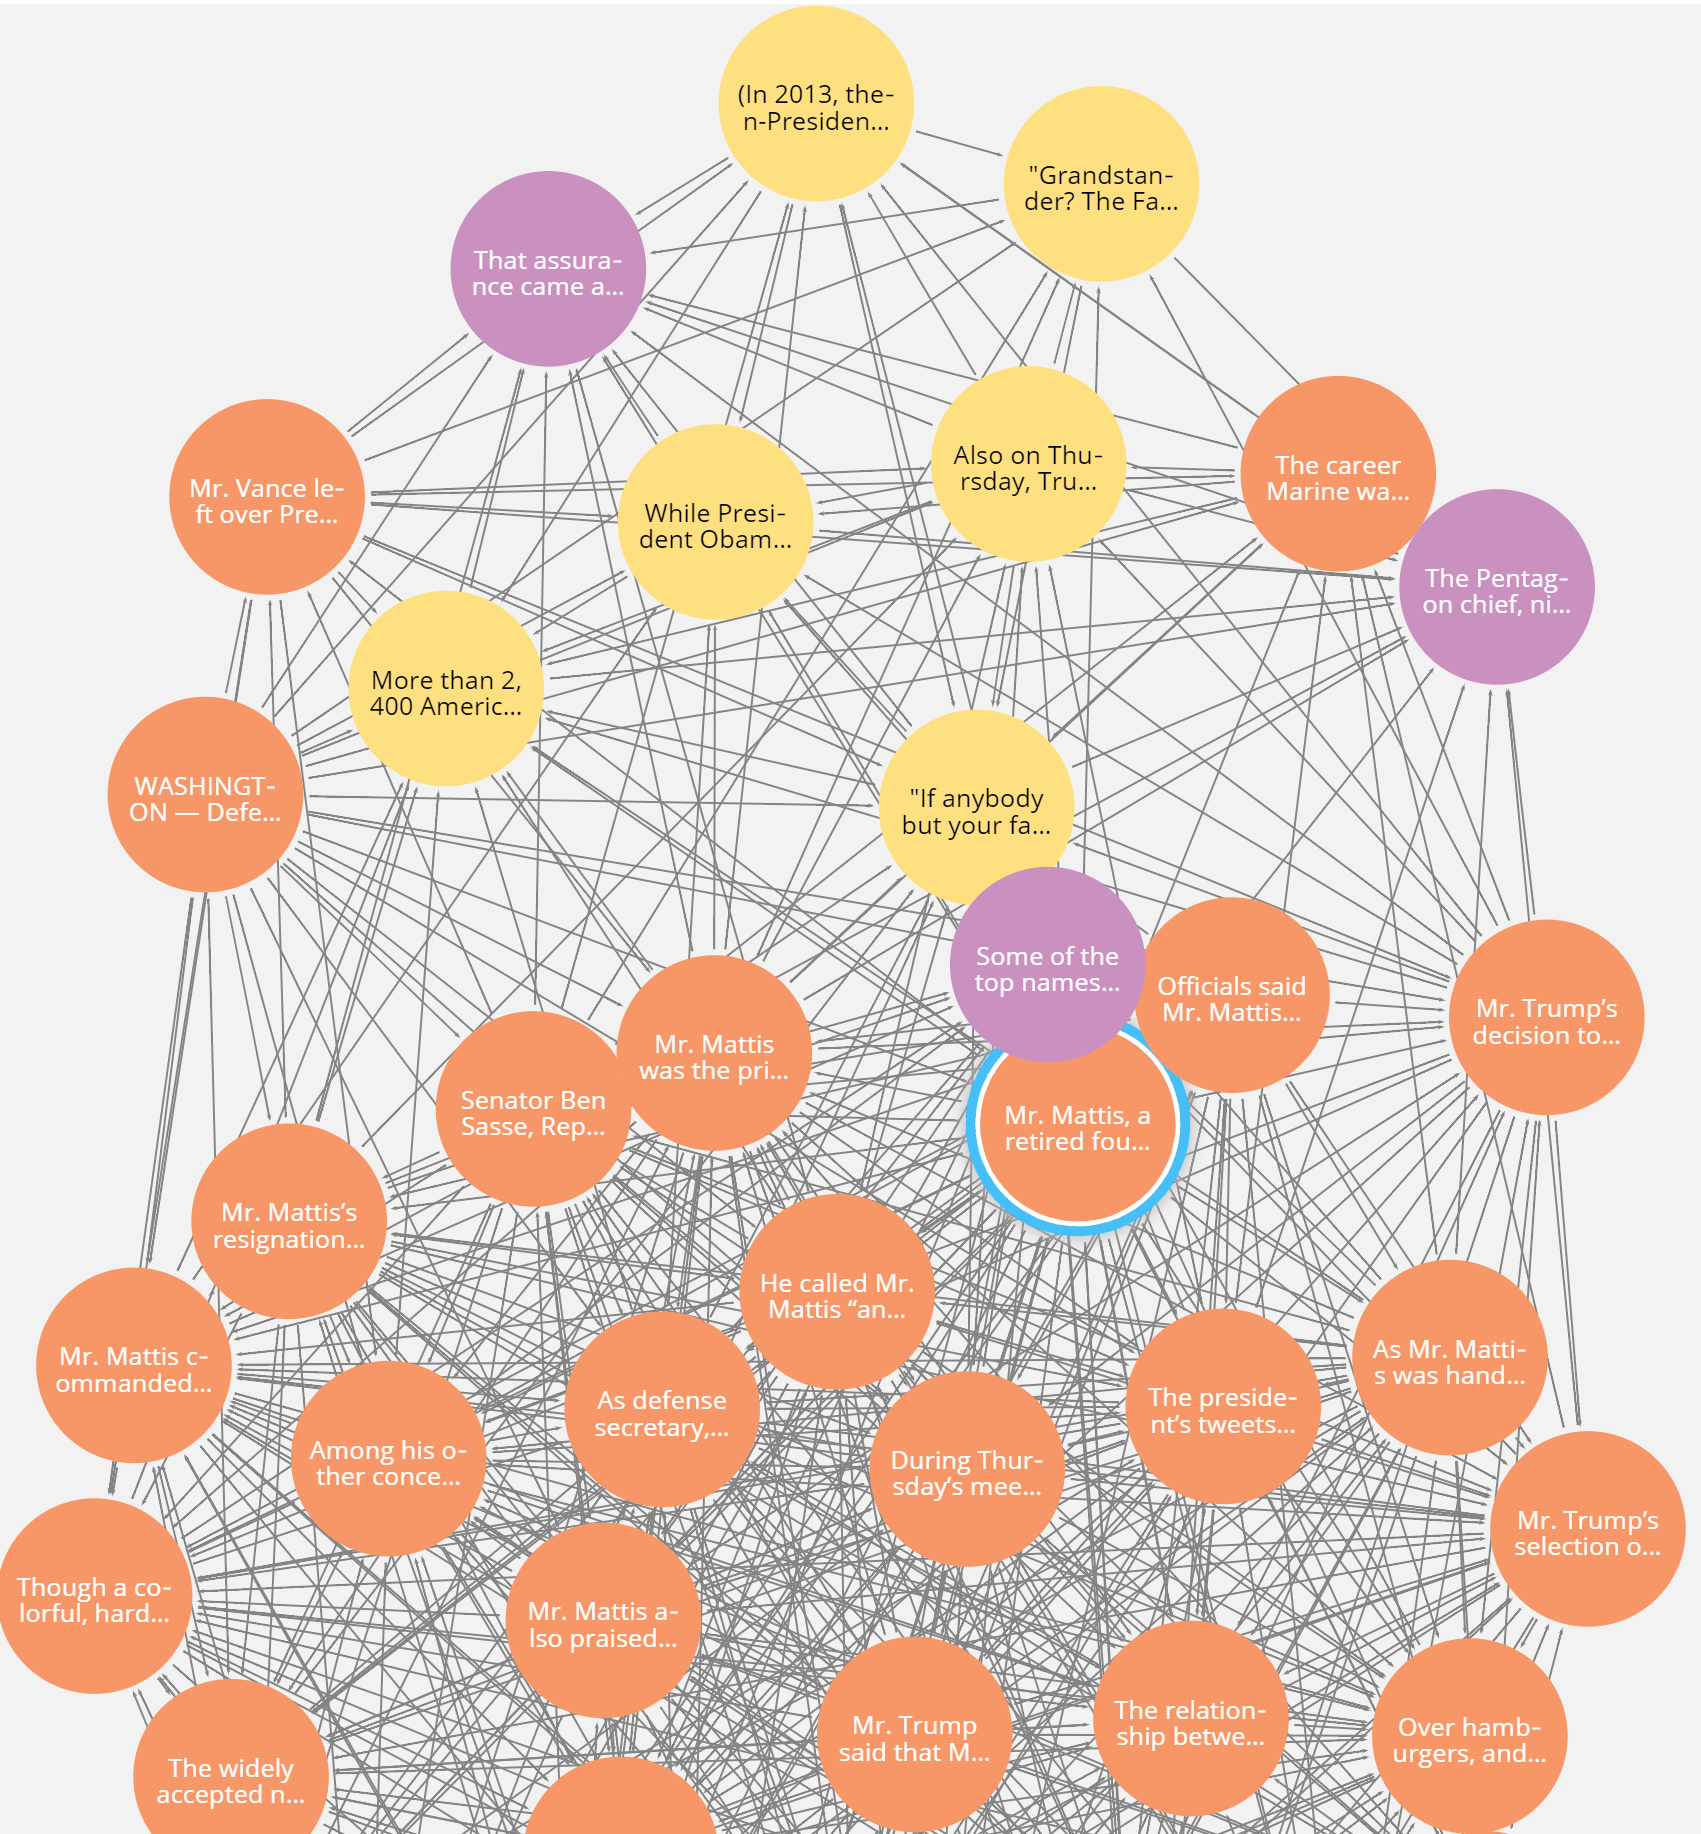
\includegraphics[width=.46\linewidth]{img/mattis0_src.png}
    \label{subfig:mattissrc}
    }
  \subfigure[nodes are colored by bias label]{
    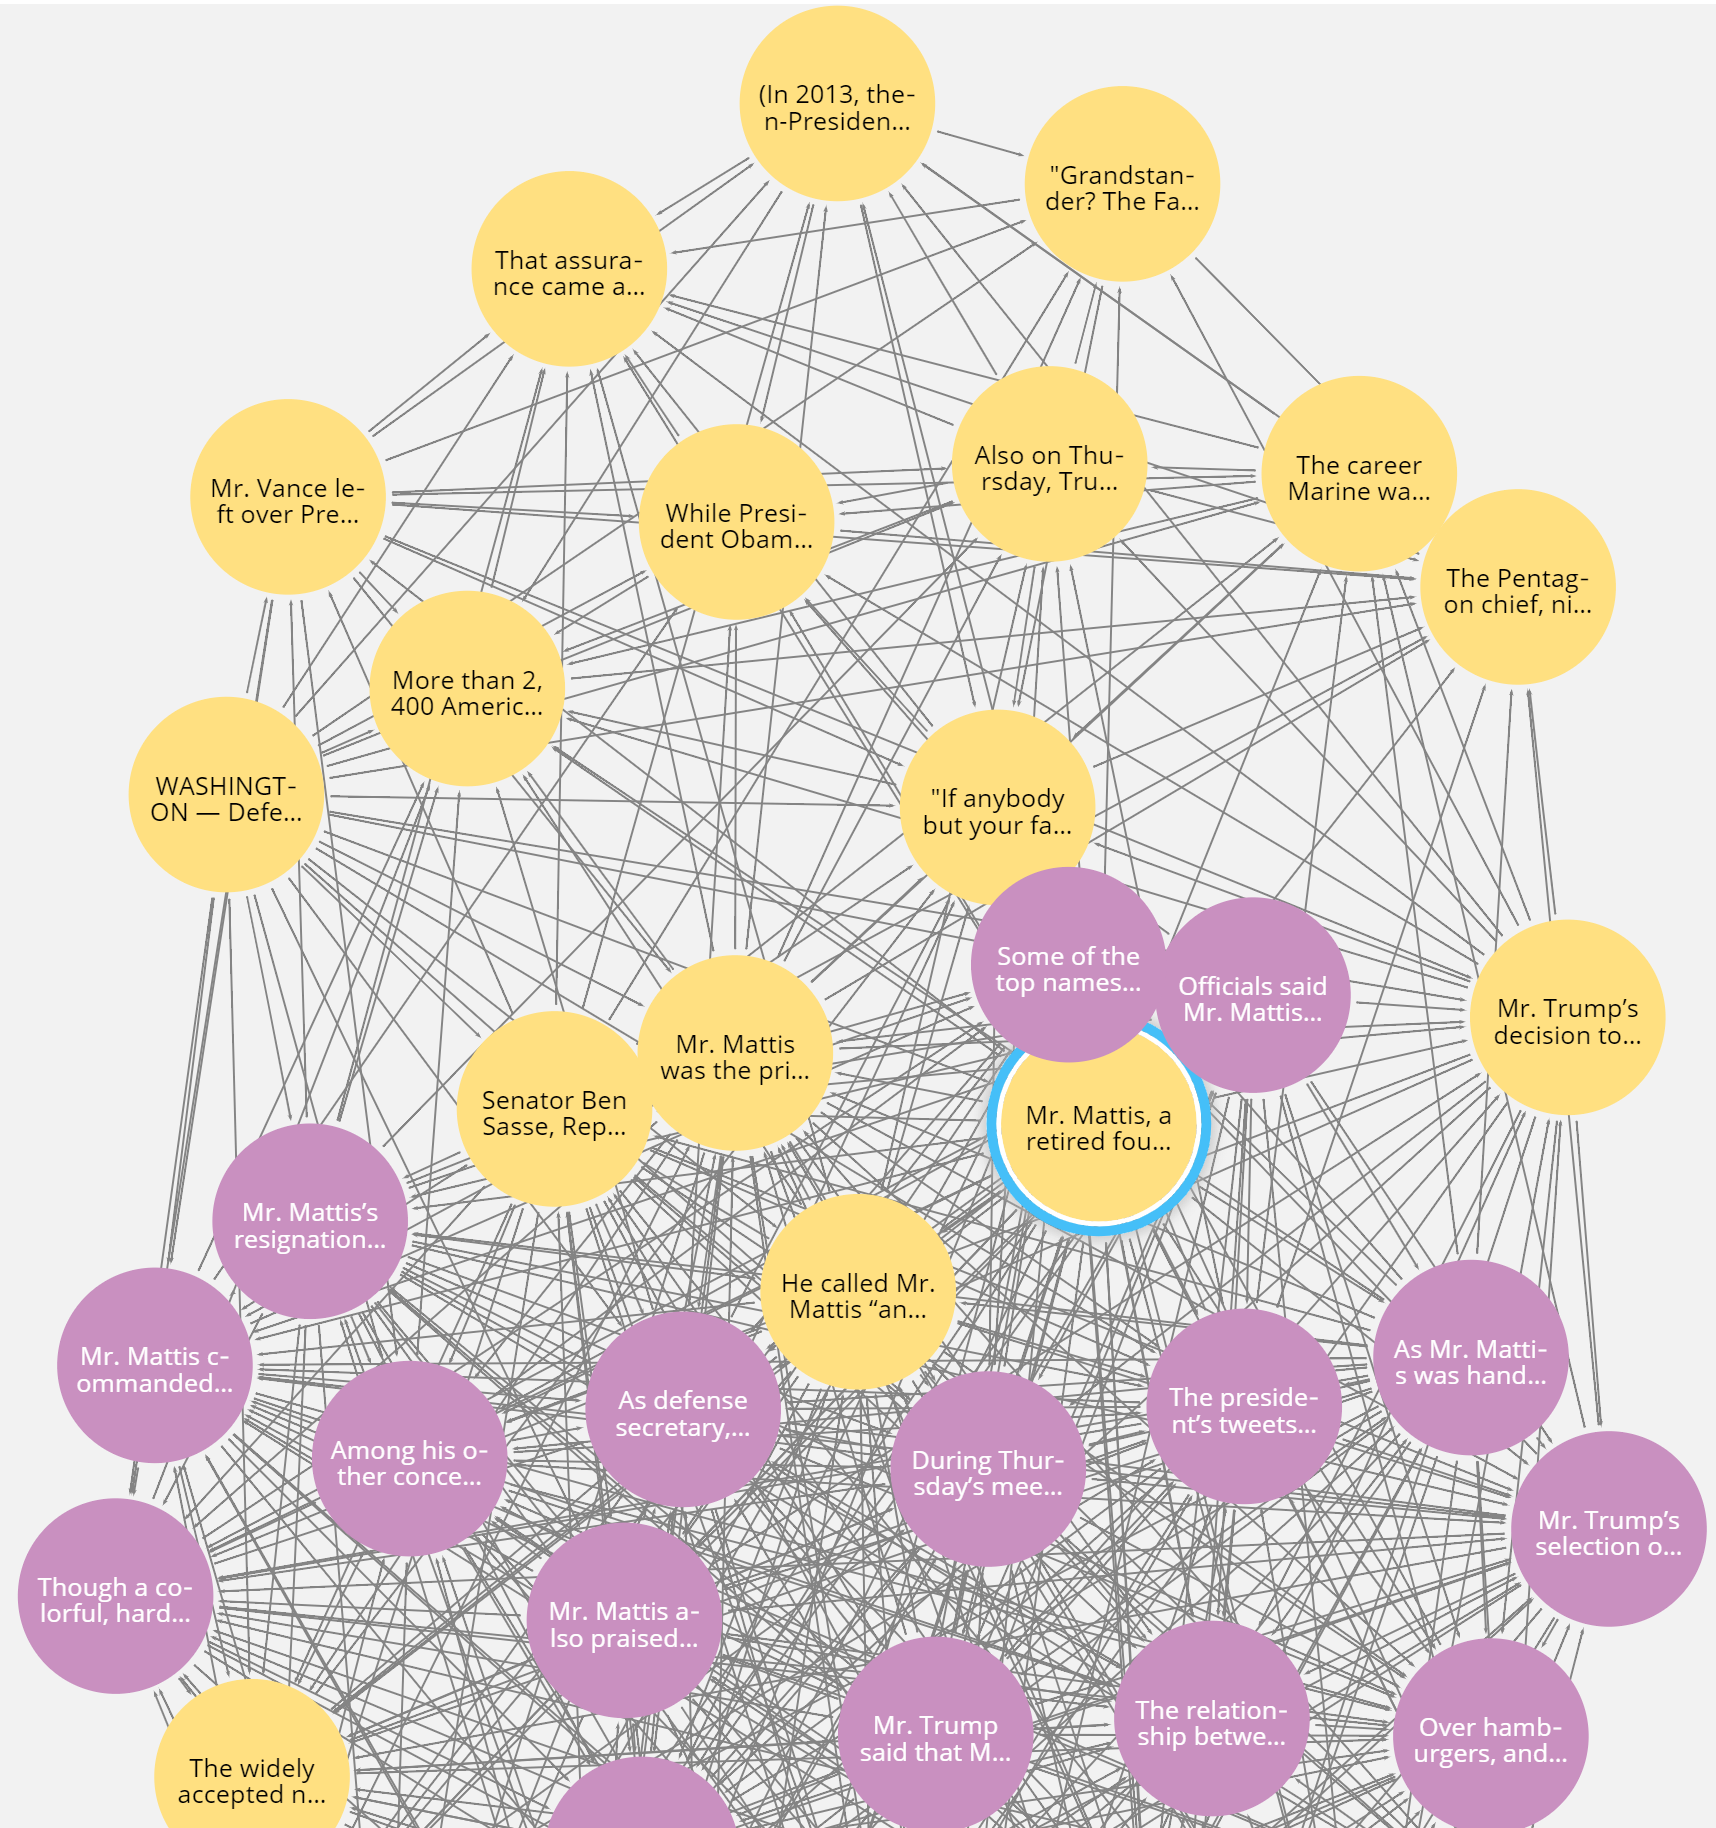
\includegraphics[width=.46\linewidth]{img/mattis0_bias.png}
    \label{subfig:mattisbias}
    }
    
%   \begin{subfigure}[t]{0.7\linewidth}
%     \resizebox{\linewidth}{!}{
%     \begin{tikzpicture}
%       [scale=.6, transform shape,
%       vertex/.style = {rounded rectangle, minimum width=60pt, minimum height = 17pt, draw = black!30, thick},
%       textbox/.style = {rectangle, minimum width=60pt, minimum height = 20pt},
%       edge_style/.style={draw=black, ultra thick}]
%         \node[vertex] (n2) at (2,6)  {\textcolor{blue!60}{The inauguration will be held very soon.} };
%     \node[vertex] (n3) at (3,2)  { .... \textbf{Trump} has also...};
%       \node[vertex][draw=blue!60, fill = blue!40] (n4) at (1,3.5)  { \textcolor{white}{\textbf{Donald Trump} is \underline{elected} president }};
%       \node[vertex] (n5) at (-2,1.7)  { \textit{However}, there's... };
%       \node[vertex] (n6) at (6,5)  {...won the \underline{election}... };
%     %   \node[textbox] at (4.5,1.3) {event A};
%       \foreach \from \to /\weight in {n4/n5/}
%         \draw[draw=black] (\from) -- node {\weight}(\to);
%     \foreach \from \to /\weight in {n4/n6/}
%         \draw[draw=black, double distance=.03cm] (\from) -- node {\weight}(\to);
%   \foreach \from \to /\weight in {n4/n2/}
%         \draw[draw=blue!60] (\from) -- node {\weight}(\to);
%   \foreach \from \to /\weight in {n4/n3/}
%         \draw[edge_style] (\from) -- node {\weight}(\to);
%     \end{tikzpicture}}
%   \caption{ Four types of edges in relational sentence graph. \underline{Underline}: deverbal noun reference; \textit{italic}: discourse maker; \textbf{bold}: entity continuation; \textcolor{blue!60}{colored}: sentence similarity}
%   \label{subfig:edgetype}
%   \end{subfigure}
%   \begin{subfigure}[t]{.35\linewidth}
%     \resizebox{\linewidth}{!}{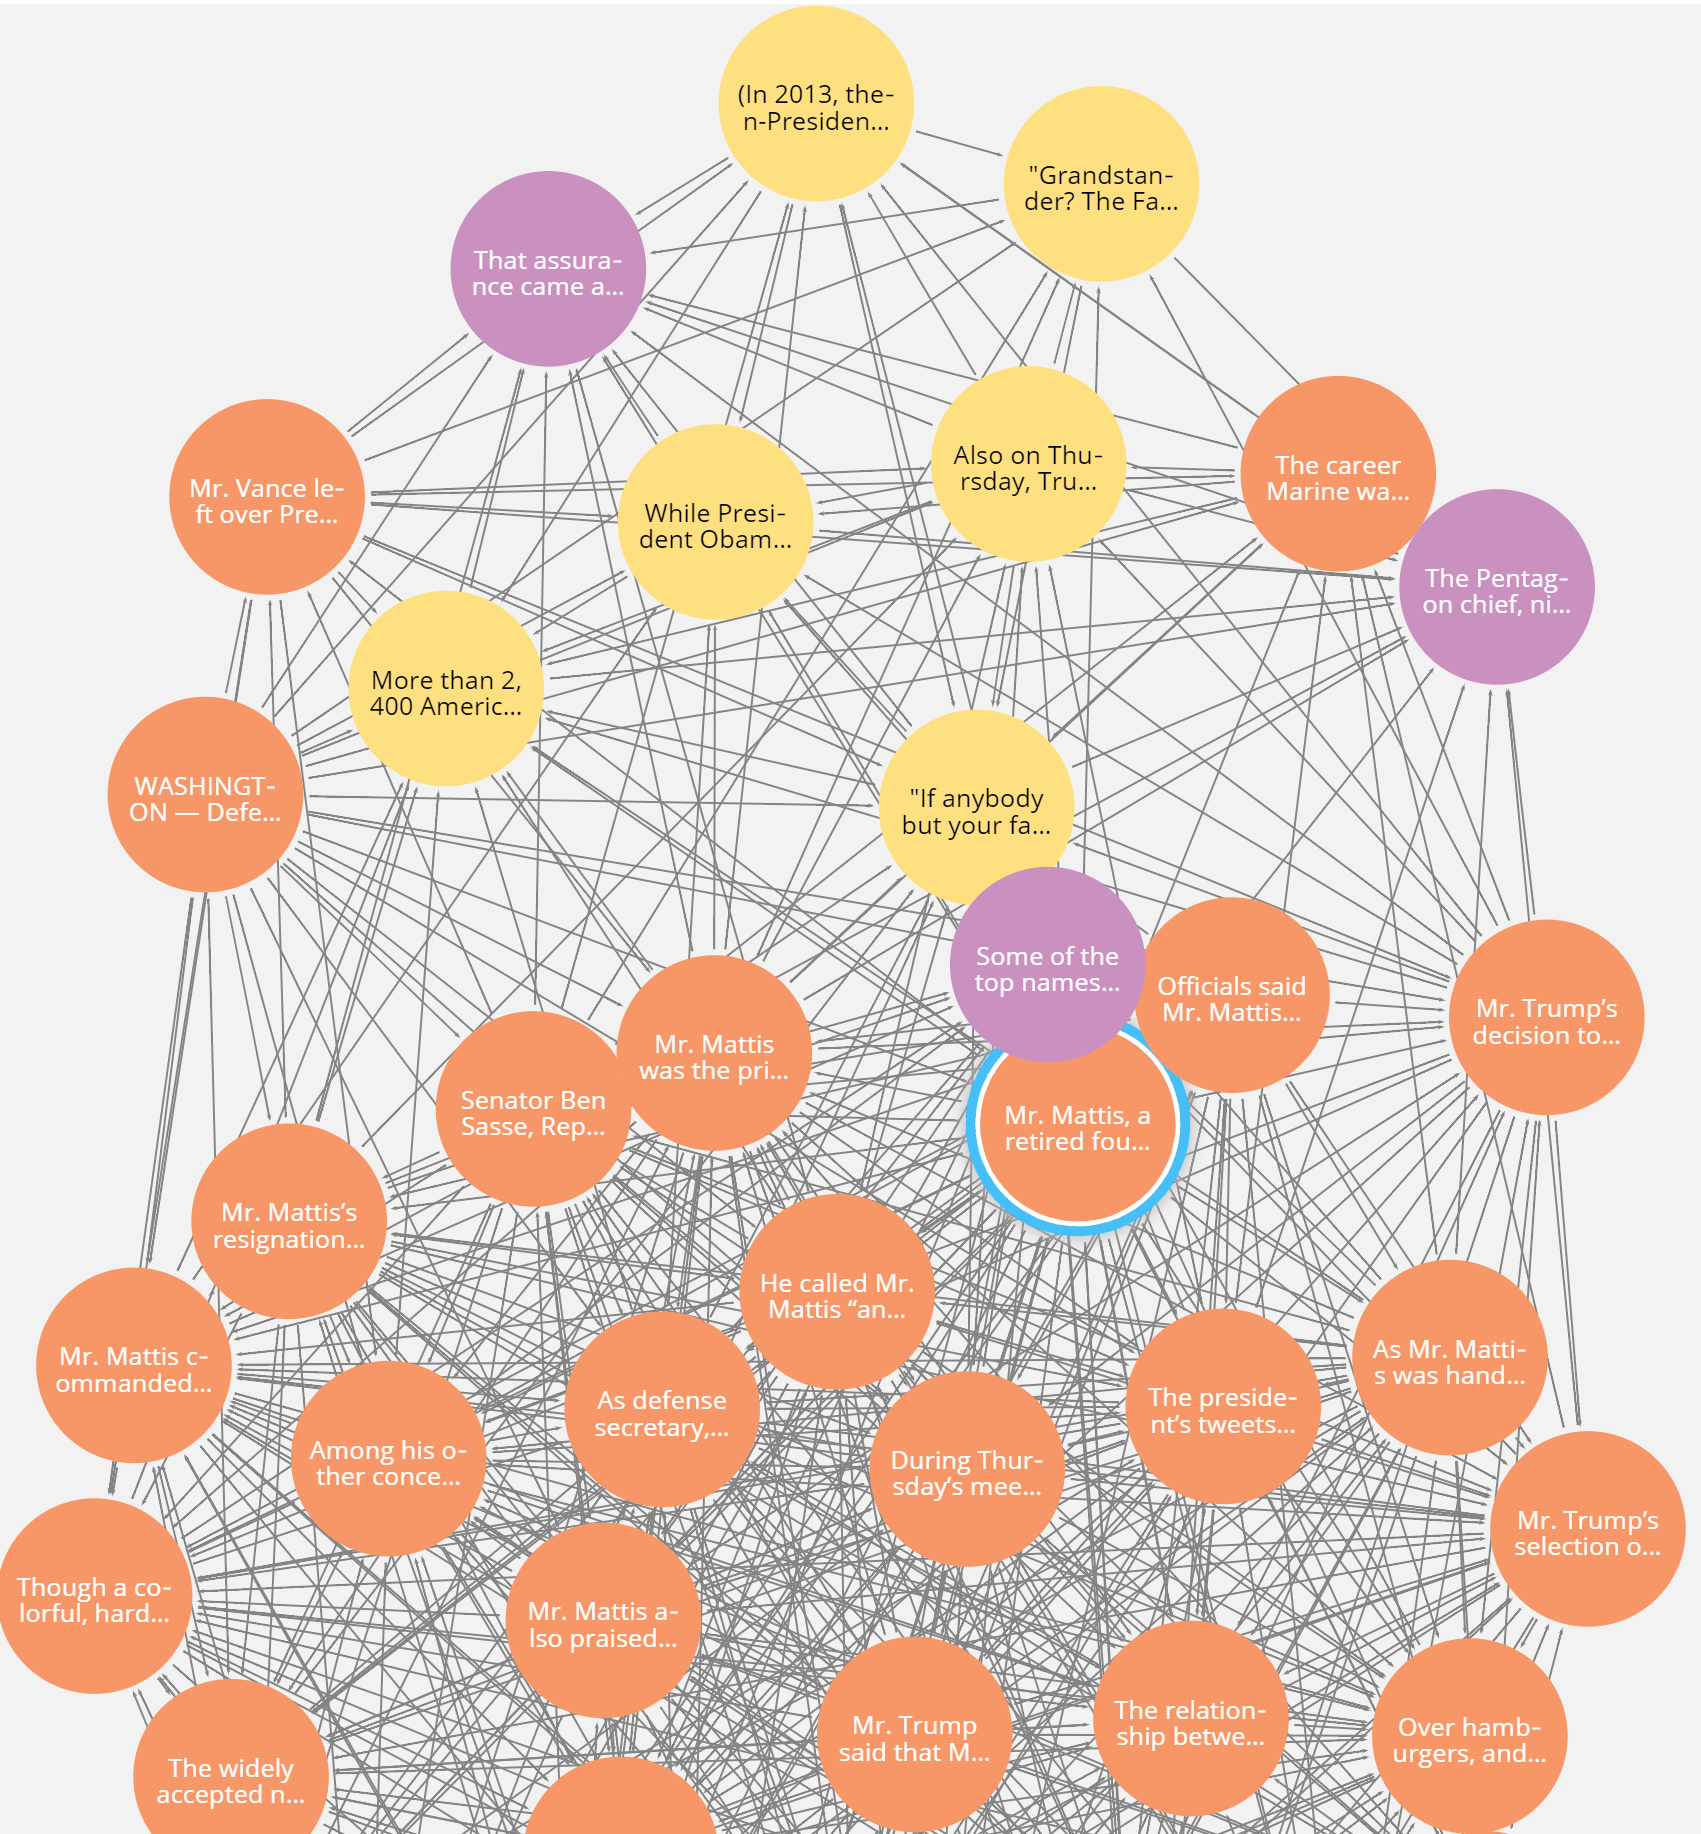
\includegraphics[]{img/mattis0_src.png}}
%     \caption{ nodes are colored by news source.}
%     \label{subfig:mattissrc}
%   \end{subfigure}
%   \begin{subfigure}[t]{.35\linewidth}
%     \resizebox{\linewidth}{!}{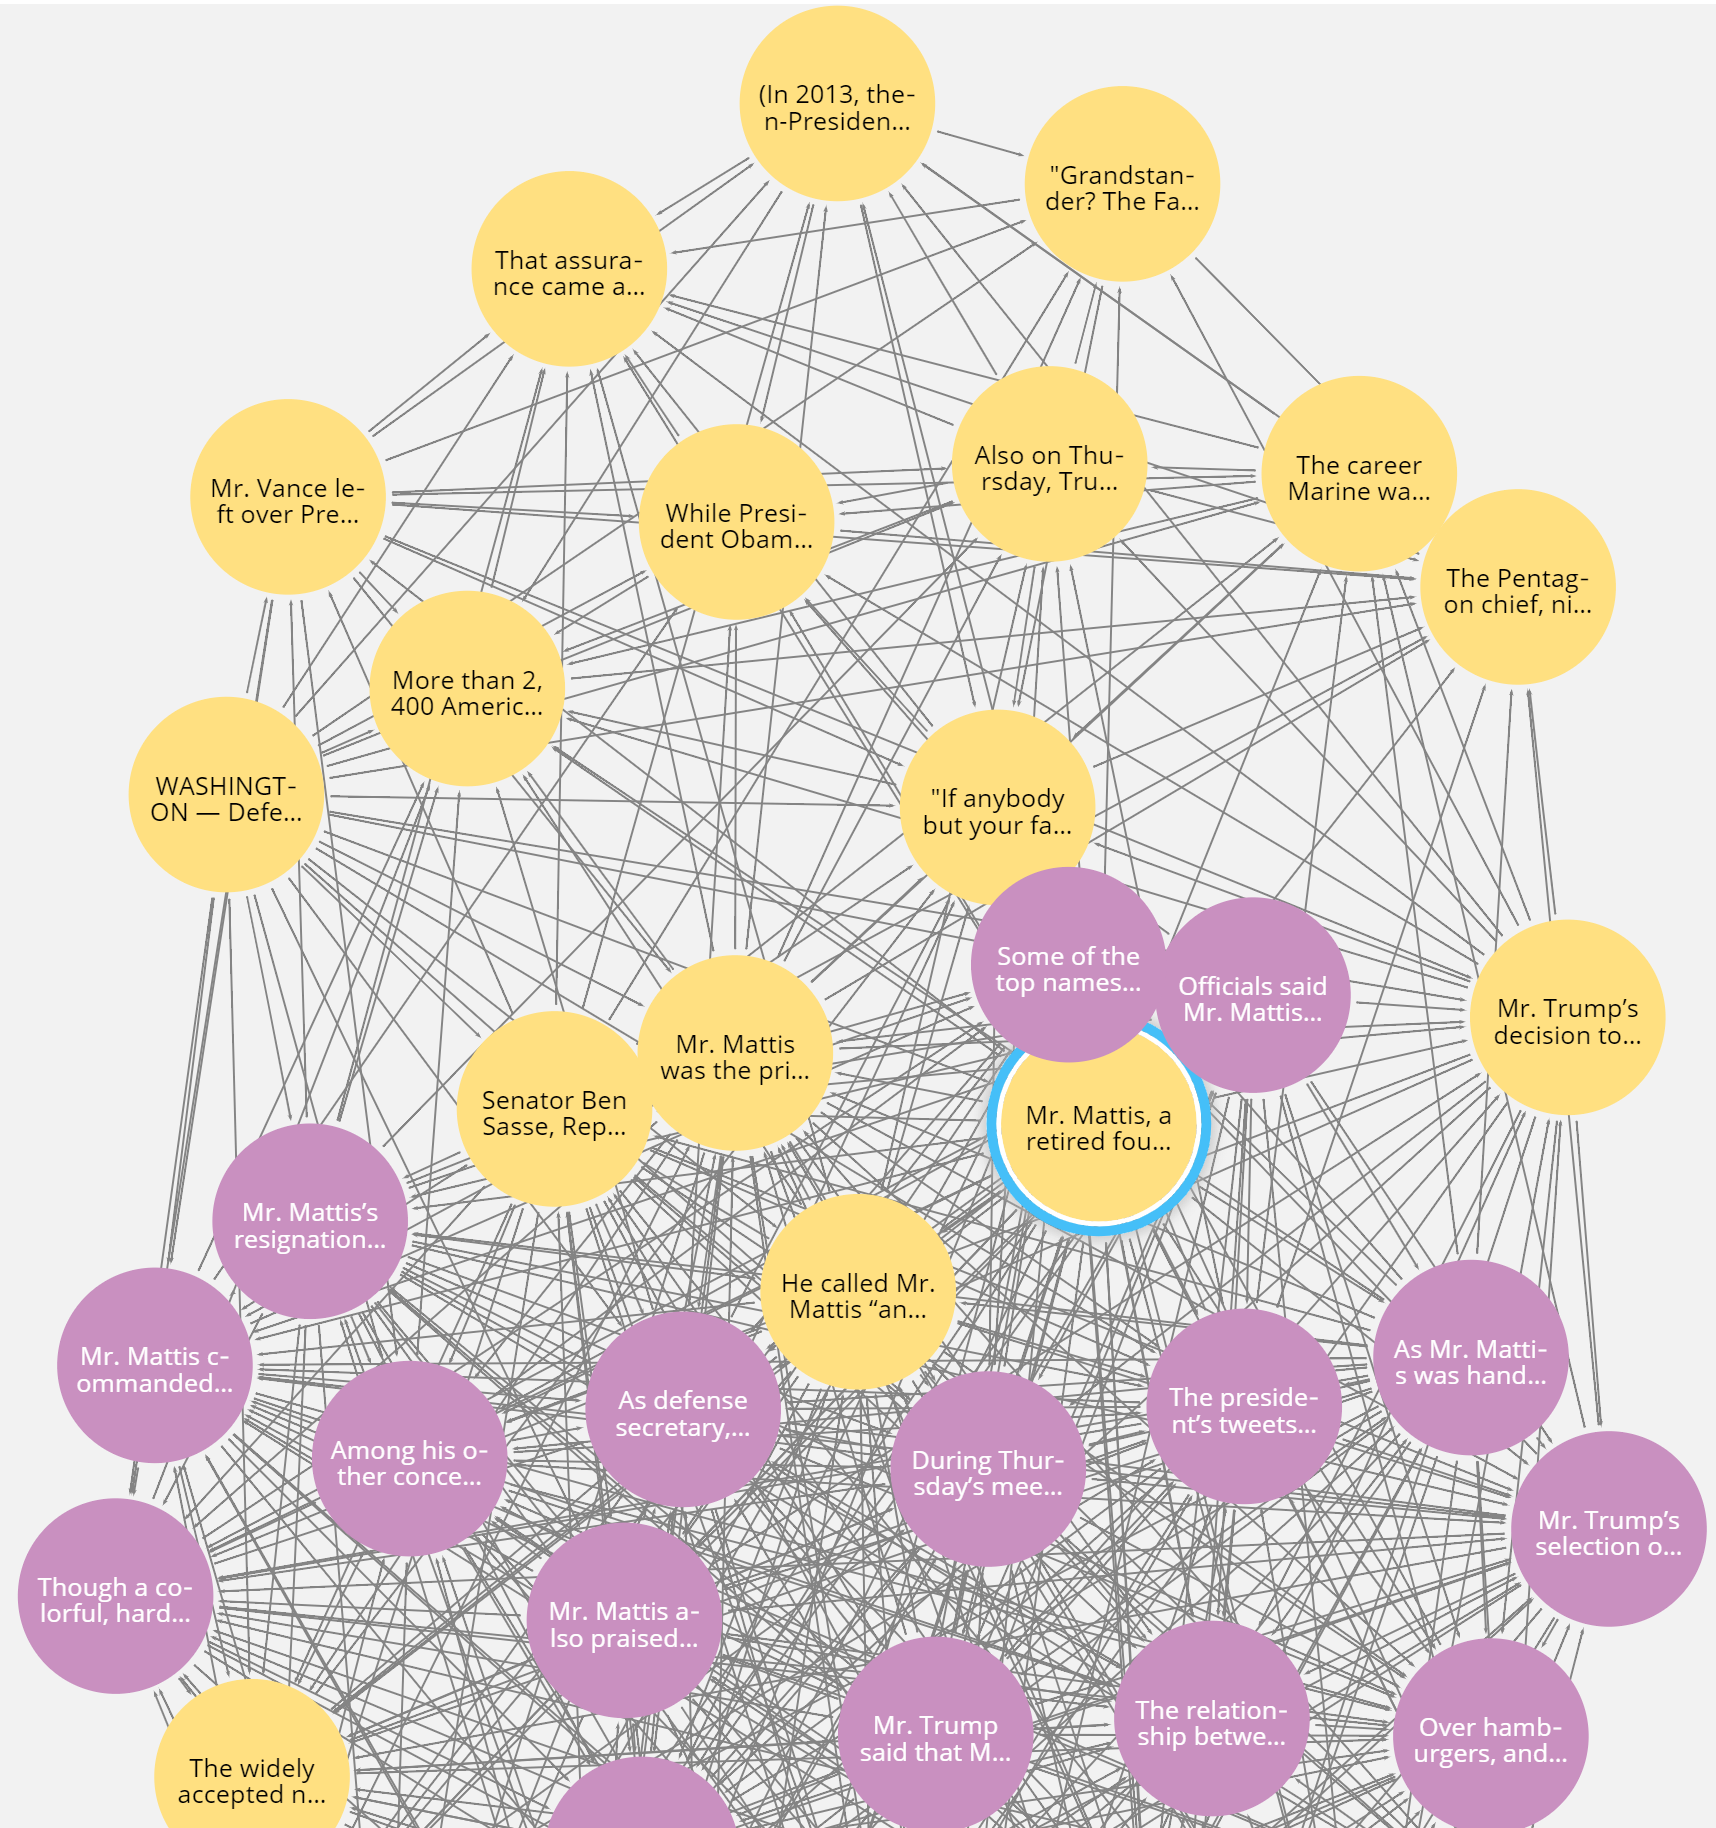
\includegraphics[]{img/mattis0_bias.png}}
%     \caption{nodes are colored by bias label.}
%     \label{subfig:mattisbias}
%   \end{subfigure}
   \caption{ Relational sentence graph} 
  \label{fig:adg}
\end{figure}



The four types of edge formation take different degrees of context into account: Type 1 and Type 2 consider only the subsequent sentences in the same article (neighborhood-context). In particular, Type 2 considers only the immediately following sentence. Type3 and Type 4 are not limited to adjacent sentences. Rather they consider the whole event (event-context). Note that edges occur only between in-event sentences, which is consistent with our event- based splitting.
% the first two types happen among only subsequent sentences in same article , especially the second one considers only the immediately following sentence; 

Figure \ref{subfig:mattissrc} and \ref{subfig:mattisbias} present the same subgraph taken directly from the real relational sentence graph in our study. We only present part of edges connected by the sentence \textit{"Mr. Mattis, a retired four-star Marine general, was rebuffed.", NYT} described in Section \ref{sent:mattis}, and the first sentence in Table \ref{tab:basil} is effectively linked to it. Moreover, nodes in Figure \ref{subfig:mattissrc} are colored according to news source (HPO/NYT/FOX) and we clearly see that relational sentence graph infuse information from different news media. In comparison of Figure \ref{subfig:mattisbias}, we found that most sentences from HPO and FOX (yellow and violet) related to target sentence are biased. Therefore event-context contained in articles of different news outlets effectively helps identify the biased sentences.

Our graph composition is intended to mimic the way humans develop views: people acquire information through immediate context in article and reason by aggregating certain background knowledge from different news reports of the whole event.

%  inspired by the Approximate Discourse Graph(ADG)
\subsection{Graph Attention Network}

As one of the representative graph convolutional networks, Graph Attention Networks (GATs) introduces an attention mechanism to achieve better neighbor aggregation. By learning the weights of the neighbors, GAT can learn the representation of the target node by implementing a weighted aggregation of the neighbor node representations. However, it may suffer from graph noise introduced by incorrect node linking. In our study, we use Self-supervised Graph Attention Network \citet{kim2021how} which introduces, on top of the GAT, an edge presence prediction task and thus puts an emphasis on more on distinguishing misconnected neighbors.

The graph structure naturally places each sentence within its context, and as a result, different sentences are no longer isolated. The flexibility of the graph structure also allows it to move beyond the ordered arrangement of traditional LSTM. Therefore two sentences can be directly connected by edges, even if they are far apart in the original article or in different articles. 
% that are far apart in the original article or even not in the same article can be directly connected by edges. 

% \KZ{One thing you need to explain is that while the relational sentence graph
% contain four different edge types, these types are not distinguished here in
% the GAN. Why? Would it be better to find a way to make such distinction?}

Note that our sentence graph doesn't contain edges between two events, therefore it assures no data leakage while training GAT on the whole graph.

%%%%%%%%model%%%%%%%%%%%%%%%%%%%%%%%%%%%%%%%%%%%%%%%%%%%%%%
\begin{figure*}[!htbp]\centering
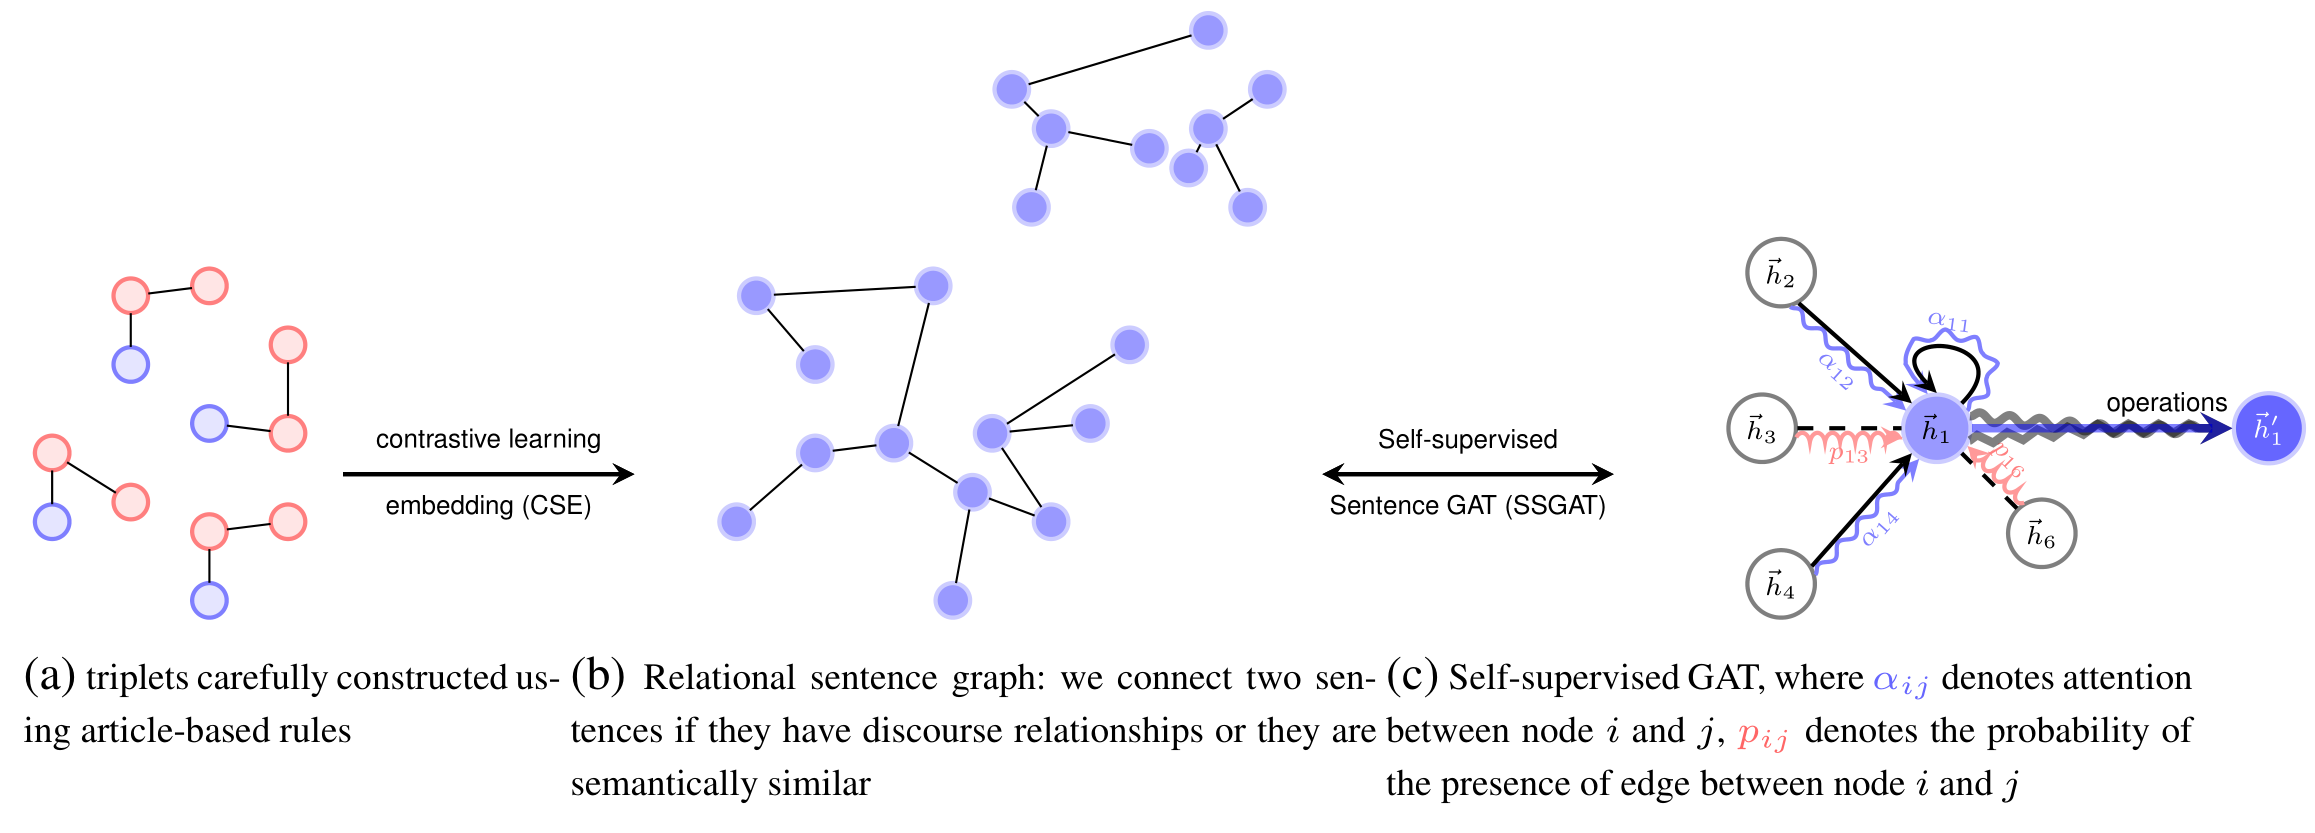
\includegraphics[width=\linewidth]{img/multictx.PNG}
% \begin{subfigure}[t]{.2\linewidth}
%   \resizebox{!}{!}{
%     \begin{tikzpicture}[scale=.13, transform shape,
%       vertex/.style = {circle, minimum width=50pt, minimum height = 17pt, draw=red!50, fill = red!10, thick},
%       neg/.style = {circle, minimum width=50pt, minimum height = 17pt, draw=blue!50, fill = blue!10, thick},
%       textbox/.style = {rectangle, minimum width=300pt, minimum height = 200pt},
%       edge_style/.style={draw=black}]
%     %   \node[event](s1) at (7,7.7) {};
%     %   \node[textbox][] at (8,4) {\huge contrastive learning};
%     \node[vertex] (n1) at (-8,7.5)  {};
%       \node[neg] (n2) at (-8,4)  {};
%       \node[vertex] (n3) at (-4,5)  {};
      
%       \node[vertex] (n4) at (0,3.5)  {};
%       \node[neg] (n5) at (0,0)  {};
%       \node[vertex] (n6) at (4,4)  {};
      
%     \node[vertex] (n7) at (-4,15.5)  {};
%       \node[neg] (n8) at (-4,12)  {};
%       \node[vertex] (n9) at (0,16)  {};
      
%       \node[vertex] (n10) at (4,8.5)  {};
%       \node[neg] (n11) at (0,9)  {};
%       \node[vertex] (n12) at (4,13)  {};
      
      
%       \foreach \from \to /\weight in {n1/n2/, n1/n3/, n4/n5/,n4/n6/, n7/n8/,n7/n9/, n10/n12/, n10/n11/}
%         \draw[edge_style] (\from) -- node {\weight}(\to);
%     \end{tikzpicture}
%     \begin{tikzpicture}[scale=.7, transform shape,
%       vertex/.style = {circle, minimum width=1pt, minimum height = 1pt, draw = white, fill = white},
%       edge_style/.style={-stealth, draw=black, thick}]
%       \node[vertex] (n1) at (-15,1.25)  {};
%     %   \node[vertex] (n2) at (10, 8.5)  {};
%      \node[vertex] (0) at (0,0) {};
%       \node[vertex] (n3) at (-12,1.25)  {};
%       \foreach \from \to /\weight in {n1/n3/}
%         \draw[edge_style] (\from) -> node[above=0.1] {contrastive learning}(\to);
%         \foreach \from \to /\weight in {n1/n3/}
%         \draw[edge_style] (\from) -> node[below=0.1] {embedding (CSE)}(\to);
%     % \foreach \from \to /\weight in {n1/n2/}
%     %     \draw[edge_style,fill=white] (\from) -> node (\to);
%     \end{tikzpicture}
%   }
%   \caption{ triplets carefully constructed using article-based rules}
% \end{subfigure}
% \begin{subfigure}[t]{.3\linewidth}
%   \resizebox{!}{!}{
%     \begin{tikzpicture}[scale=.13, transform shape,
%       event/.style = {rounded rectangle, minimum width=300pt, minimum height = 600pt, draw = black, fill = white, thick},
%       vertex/.style = {circle, minimum width=50pt, minimum height = 50pt, draw =blue!20, fill = blue!40, thick},
%       textbox/.style = {rectangle, minimum width=60pt, minimum height = 20pt},
%       edge_style/.style={draw=black}]
%     \node[vertex][draw=white,fill=white] (0) at (-15,0) {};
    
%     \node[vertex] (n1) at (-4,7.5)  {};
%       \node[vertex](n2) at (-8,4)  {};
%       \node[vertex] (n3) at (0,8)  {};
      
%       \node[vertex] (n4) at (4,5.5)  {};
%       \node[vertex] (n5) at (3,0)  {};
%       \node[vertex] (n6) at (8,4)  {};
      
%     \node[vertex] (n7) at (-7,15.5)  {};
%       \node[vertex] (n8) at (-4,12)  {};
%       \node[vertex] (n9) at (2,16)  {};
      
%     \node[vertex] (n10) at (5,8.5)  {};
%       \node[vertex] (n11) at (10,9)  {};
%       \node[vertex] (n12) at (12,13)  {};
      
      
%         \node[vertex] (p4) at (8,24)  {};
%       \node[vertex] (p5) at (13,23)  {};
%       \node[vertex] (p6) at (6,26)  {};
      
%     \node[vertex] (p7) at (16,24)  {};
%       \node[vertex] (p8) at (15,22)  {};
%       \node[vertex] (p9) at (19,26)  {};
      
%     \node[vertex] (p10) at (16,29)  {};
%       \node[vertex] (p11) at (18,20)  {};
%       \node[vertex] (p12) at (7,20)  {};
      
%     %   \node[textbox] at (4.5,1.3) {triplets};
%       \foreach \from \to /\weight in {n1/n2/, n1/n3/,n3/n4/,n3/n9/, n4/n5/,n4/n6/, n7/n8/,n7/n9/, n10/n6/, n11/n10/,n12/n10/, p4/p5/,p4/p6/, p7/p8/,p7/p9/, p10/p6/, p11/p7/,p12/p4/}
%         \draw[edge_style] (\from) -- node {\weight}(\to);
%     \end{tikzpicture}
%     % 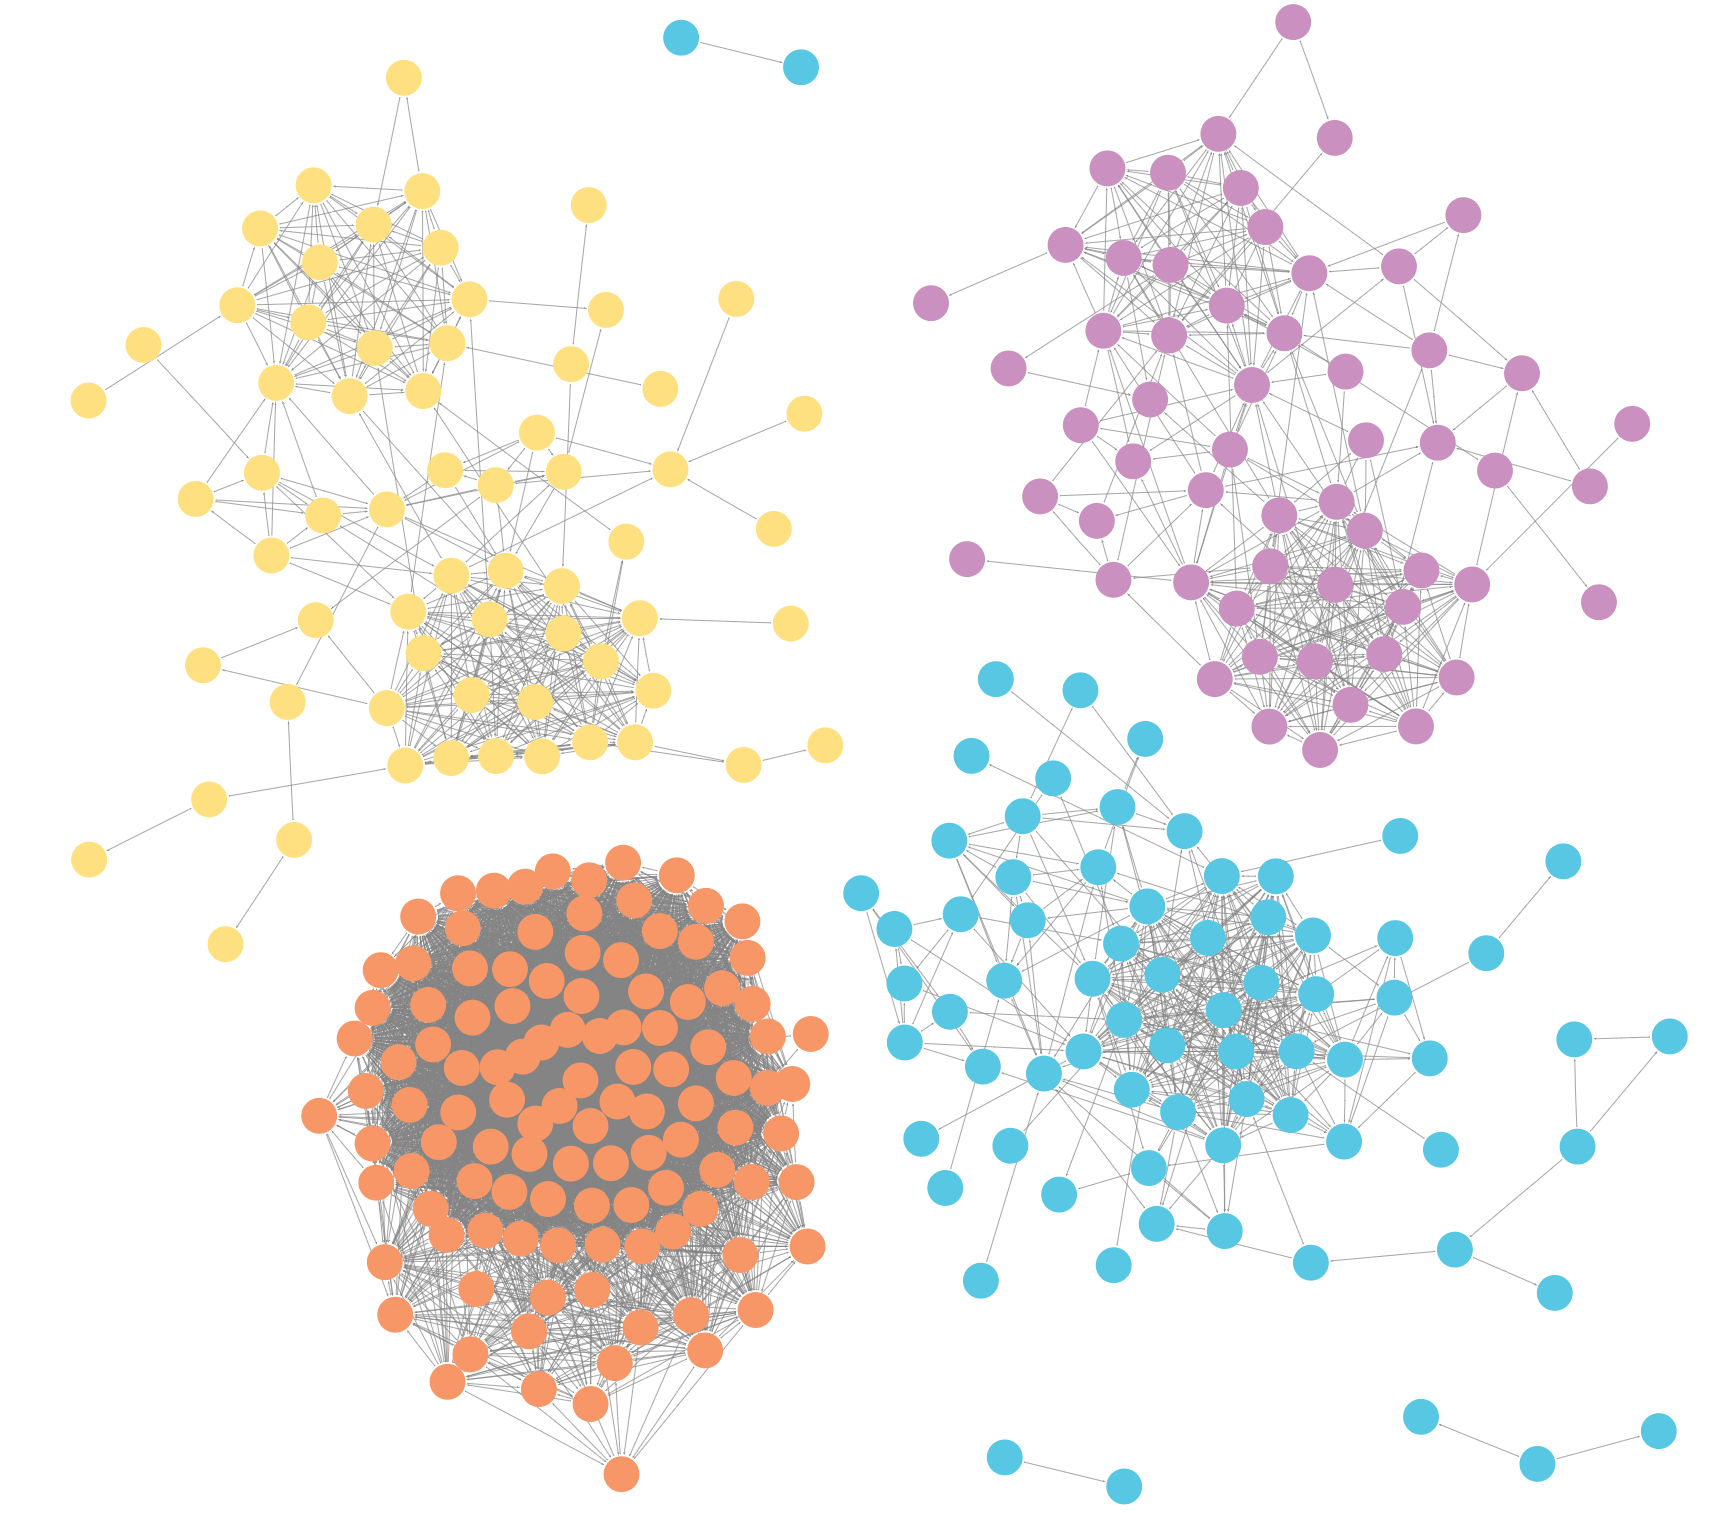
\includegraphics[]{img/sample.png}
%     \begin{tikzpicture}[scale=.7, transform shape,
%       vertex/.style = {circle, minimum width=1pt, minimum height = 1pt, draw = white, fill = white},
%       edge_style/.style={stealth-stealth, draw=black, thick}]
%       \node[vertex] (n1) at (-6,1.25)  {};
%      \node[vertex] (0) at (100,0) {};
%       \node[vertex] (n3) at (-3,1.25)  {};
%       \foreach \from \to /\weight in {n1/n3/}
%         \draw[edge_style] (\from) -> node[above=0.1] {Self-supervised }(\to);
%     \foreach \from \to /\weight in {n1/n3/}
%         \draw[edge_style] (\from) -> node[below=0.1] {Sentence GAT (SSGAT)}(\to);
%     \end{tikzpicture}
%   }
%   \caption{ Relational sentence graph: we connect two sentences if they have discourse relationships or they are semantically similar}
% \end{subfigure}
% \begin{subfigure}[t]{.3\linewidth}
%   \resizebox{!}{!}{
%     \begin{tikzpicture}[scale=.7, transform shape,
%       event/.style = {rounded rectangle, minimum width=300pt, minimum height = 600pt, draw = black, fill = white, thick},
%       vertex/.style = {rounded rectangle, minimum width=60pt, minimum height = 40pt, draw = black, fill = green!15, thick},
%       textbox/.style = {rectangle, minimum width=60pt, minimum height = 20pt},
%       edge_style/.style={draw=black, thick}]
%   \node[circle] (0) at (-5,0) {};
% 	\node[circle, draw=blue!20, fill = blue!40, thick] (h1) {$\vec{h}_1$};
% 	\node[circle,draw=blue!20, fill = blue!60, thick, right=10em of h1, opacity=1] (hp) {\textcolor{white}{$\vec{h}_1'$}};
% 	\node[circle, draw=black!50, thick, above left=of h1] (h4) {$\vec{h}_2$};
% 	\node[circle, draw=black!50, thick, left=4em of h1] (h5) {$\vec{h}_3$};
% 	\node[circle, draw=black!50, thick, below left=of h1] (h6) {$\vec{h}_4$};
% % 	\node[circle, draw, thick, below=5em of h1] (h7) {$\vec{h}_5$};
% 	\node[circle, draw=black!50, thick, below right=3em of h1] (h8) {$\vec{h}_6$};
	
% 	\draw[-stealth, red!40,thick,decoration={coil,amplitude=0.3mm,segment length=1mm}, decorate] (h8.120) -- node[sloped, above, black] {\textcolor{red!50}{$p_{16}$}} (h1.-30);
% 	\draw[dashed, thick] (h8.135) -- (h1.-45);
% % 	\draw[-stealth, mygreen, thick, decoration={zigzag, pre length=0.01mm, segment length=2mm, amplitude=0.3mm, post length=1.5mm}, decorate] (h8.150) -- (h1.-60);
	
% 	\draw[-stealth, blue!50, thick,decoration={snake, pre length=0.01mm, segment length=2mm, amplitude=0.3mm, post length=1.5mm}, decorate] (h1.30) to[looseness=7] node[sloped, above, black] {\textcolor{blue!50}{${\alpha}_{11}$}}(h1.105);
% 	\draw[-stealth, thick] (h1.45) to[looseness=9] (h1.90);
% % 	\draw[-stealth, mygreen, thick, decoration={zigzag, pre length=0.01mm, segment length=2mm, amplitude=0.3mm, post length=1.5mm}, decorate] (h1.60) to[looseness=20] (h1.75);
	
% 	\draw[-stealth, blue!50, thick,decoration={snake, pre length=0.01mm, segment length=2mm, amplitude=0.3mm, post length=1.5mm}, decorate] (h4.285) -- node[sloped, below, black] {\textcolor{blue!50}{${\alpha}_{12}$}}(h1.150);
% 	\draw[-stealth,  thick] (h4.300) -- (h1.135);
% % 	\draw[-stealth, mygreen, thick, decoration={zigzag, pre length=0.01mm, segment length=2mm, amplitude=0.3mm, post length=1.5mm}, decorate] (h4.315) -- (h1.120);
	
% 	\draw[-stealth, red!40, thick,decoration={coil,amplitude=0.3mm,segment length=1mm}, decorate] (h5.-15) -- node[sloped, below, black] {\textcolor{red!50}{$p_{13}$}}(h1.195);
% 	\draw[dashed, thick] (h5.0) -- (h1.180);
% % 	\draw[-stealth, mygreen, thick, decoration={zigzag, pre length=0.01mm, segment length=2mm, amplitude=0.3mm, post length=1.5mm}, decorate] (h5.15) -- (h1.165);
	
% 	\draw[-stealth, blue!50, thick,decoration={snake, pre length=0.01mm, segment length=2mm, amplitude=0.3mm, post length=1.5mm}, decorate] (h6.15) -- node[sloped, below, black] {\textcolor{blue!50}{${\alpha}_{14}$}}(h1.240);
% 	\draw[-stealth, thick] (h6.30) -- (h1.225);
% % 	\draw[-stealth, mygreen, thick, decoration={zigzag, pre length=0.01mm, segment length=2mm, amplitude=0.3mm, post length=1.5mm}, decorate] (h6.45) -- (h1.210);
	
% % 	\draw[-stealth, mymauve, thick,decoration={snake, pre length=0.01mm, segment length=2mm, amplitude=0.3mm, post length=1.5mm}, decorate] (h7.75) -- node[sloped, below, black] {$\vec{\alpha}_{15}$}(h1.-75);
% % 	\draw[-stealth, dashed, thick] (h7.90) -- (h1.-90);
% % 	\draw[-stealth, mygreen, thick, decoration={zigzag, pre length=0.01mm, segment length=2mm, amplitude=0.3mm, post length=1.5mm}, decorate] (h7.105) -- (h1.-105);
	

	
% 	\coordinate[right=5em of h1] (A);
	
% 	\draw[-stealth,  opacity=0.5, ultra thick,decoration={snake, pre length=0.01mm, segment length=2mm, amplitude=0.3mm, post length=1.5mm}, decorate] (h1.20) -- (A) -- (hp);
% 	\draw[-stealth, opacity=0.5, ultra thick,decoration={zigzag, pre length=0.01mm, segment length=2mm, amplitude=0.3mm, post length=1.5mm}, decorate] (h1.-20) -- (A) -- (hp);
% 	\draw[-stealth, blue, opacity=0.5, ultra thick] (h1.0) -- (A) -- node[black, above, opacity=1.0] {operations} (hp);
%     \end{tikzpicture}
%   }
%     \caption{ Self-supervised GAT, where \textcolor{blue!60}{$\alpha_{ij}$} denotes attention between node $i$ and $j$, \textcolor{red!60}{$p_{ij}$} denotes the probability of the presence of edge between node $i$ and $j$}
% \end{subfigure}
  \caption{ Our Model MultiCTX }
  \label{fig:model}
\end{figure*}